\documentclass[twoside]{book}

% Packages required by doxygen
\usepackage{fixltx2e}
\usepackage{calc}
\usepackage{doxygen}
\usepackage[export]{adjustbox} % also loads graphicx
\usepackage{graphicx}
\usepackage[utf8]{inputenc}
\usepackage{makeidx}
\usepackage{multicol}
\usepackage{multirow}
\PassOptionsToPackage{warn}{textcomp}
\usepackage{textcomp}
\usepackage[nointegrals]{wasysym}
\usepackage[table]{xcolor}

% Font selection
\usepackage[T1]{fontenc}
\usepackage[scaled=.90]{helvet}
\usepackage{courier}
\usepackage{amssymb}
\usepackage{sectsty}
\renewcommand{\familydefault}{\sfdefault}
\allsectionsfont{%
  \fontseries{bc}\selectfont%
  \color{darkgray}%
}
\renewcommand{\DoxyLabelFont}{%
  \fontseries{bc}\selectfont%
  \color{darkgray}%
}
\newcommand{\+}{\discretionary{\mbox{\scriptsize$\hookleftarrow$}}{}{}}

% Page & text layout
\usepackage{geometry}
\geometry{%
  a4paper,%
  top=2.5cm,%
  bottom=2.5cm,%
  left=2.5cm,%
  right=2.5cm%
}
\tolerance=750
\hfuzz=15pt
\hbadness=750
\setlength{\emergencystretch}{15pt}
\setlength{\parindent}{0cm}
\setlength{\parskip}{3ex plus 2ex minus 2ex}
\makeatletter
\renewcommand{\paragraph}{%
  \@startsection{paragraph}{4}{0ex}{-1.0ex}{1.0ex}{%
    \normalfont\normalsize\bfseries\SS@parafont%
  }%
}
\renewcommand{\subparagraph}{%
  \@startsection{subparagraph}{5}{0ex}{-1.0ex}{1.0ex}{%
    \normalfont\normalsize\bfseries\SS@subparafont%
  }%
}
\makeatother

% Headers & footers
\usepackage{fancyhdr}
\pagestyle{fancyplain}
\fancyhead[LE]{\fancyplain{}{\bfseries\thepage}}
\fancyhead[CE]{\fancyplain{}{}}
\fancyhead[RE]{\fancyplain{}{\bfseries\leftmark}}
\fancyhead[LO]{\fancyplain{}{\bfseries\rightmark}}
\fancyhead[CO]{\fancyplain{}{}}
\fancyhead[RO]{\fancyplain{}{\bfseries\thepage}}
\fancyfoot[LE]{\fancyplain{}{}}
\fancyfoot[CE]{\fancyplain{}{}}
\fancyfoot[RE]{\fancyplain{}{\bfseries\scriptsize Generated by Doxygen }}
\fancyfoot[LO]{\fancyplain{}{\bfseries\scriptsize Generated by Doxygen }}
\fancyfoot[CO]{\fancyplain{}{}}
\fancyfoot[RO]{\fancyplain{}{}}
\renewcommand{\footrulewidth}{0.4pt}
\renewcommand{\chaptermark}[1]{%
  \markboth{#1}{}%
}
\renewcommand{\sectionmark}[1]{%
  \markright{\thesection\ #1}%
}

% Indices & bibliography
\usepackage{natbib}
\usepackage[titles]{tocloft}
\setcounter{tocdepth}{3}
\setcounter{secnumdepth}{5}
\makeindex

% Hyperlinks (required, but should be loaded last)
\usepackage{ifpdf}
\ifpdf
  \usepackage[pdftex,pagebackref=true]{hyperref}
\else
  \usepackage[ps2pdf,pagebackref=true]{hyperref}
\fi
\hypersetup{%
  colorlinks=true,%
  linkcolor=blue,%
  citecolor=blue,%
  unicode%
}

% Custom commands
\newcommand{\clearemptydoublepage}{%
  \newpage{\pagestyle{empty}\cleardoublepage}%
}

\usepackage{caption}
\captionsetup{labelsep=space,justification=centering,font={bf},singlelinecheck=off,skip=4pt,position=top}

%===== C O N T E N T S =====

\begin{document}

% Titlepage & ToC
\hypersetup{pageanchor=false,
             bookmarksnumbered=true,
             pdfencoding=unicode
            }
\pagenumbering{roman}
\begin{titlepage}
\vspace*{7cm}
\begin{center}%
{\Large Research Track -\/ first assignment }\\
\vspace*{1cm}
{\large Generated by Doxygen 1.8.11}\\
\end{center}
\end{titlepage}
\clearemptydoublepage
\tableofcontents
\clearemptydoublepage
\pagenumbering{arabic}
\hypersetup{pageanchor=true}

%--- Begin generated contents ---
\chapter{Research Track I -\/ first assignment}
\label{md__root_Desktop_assignmentRT_github_myfirstassignment_README}
\hypertarget{md__root_Desktop_assignmentRT_github_myfirstassignment_README}{}
In this first assignment we were asked to control an holonomic robot within a 2d space with a simple 2d simulator, Stage. The simulator can be launched by executing the command\+:


\begin{DoxyCode}
1 rosrun stage\_ros stageros $(rospack find assignment1)/world/exercise.world
\end{DoxyCode}


\section*{How the project is structured}

Once I have created a new R\+OS package, {\bfseries two R\+OS nodes} have been developed. For writing the code I have chosen to adopt C++ programming language.

\subsection*{The first node}

The first node, \href{https://github.com/fedehub/myfirstassignment/blob/main/src/random_movement.cpp}{\tt random\+\_\+movement.\+cpp}, implement\+:


\begin{DoxyEnumerate}
\item A R\+OS publisher
\item A R\+OS subscriber
\item A R\+OS client
\end{DoxyEnumerate}

\subsection*{The second node}

The second node \href{https://github.com/fedehub/myfirstassignment/blob/main/src/random_service.cpp}{\tt random\+\_\+service.\+cpp}, implement a server whose aim is to compute 2 random numbers

\subsection*{The rdm.\+srv file}

It is visible in the \href{https://github.com/fedehub/myfirstassignment/blob/main/srv/}{\tt srv} folder and it manages the request/reply of the custom service

\subsection*{Documentation}

The documentation of this project, obtained by means of {\bfseries Doxy\+Gen} is visible, within the \href{https://github.com/fedehub/myfirstassignment/blob/main/docs}{\tt docs} folder

\section*{How to launch}


\begin{DoxyEnumerate}
\item Firstly, create a folder named \+\_\+\char`\"{}myfirstassignment\char`\"{}\+\_\+
\item Within the aforementioned folder, open the terminal and run 
\begin{DoxyCode}
1 git clone https://github.com/fedehub/myfirstassignment/
\end{DoxyCode}

\item Then, to launch the simulation enviroment, please run the comamnd 
\begin{DoxyCode}
1 rosrun stage\_ros stageros $(rospack find assignment1)/world/exercise.world
\end{DoxyCode}

\item To launch the \href{https://github.com/fedehub/myfirstassignment/blob/main/src/random_movement.cpp}{\tt firs node}, digit\+:
\end{DoxyEnumerate}


\begin{DoxyCode}
1 rosrun myfirstassignment rand\_ser 
\end{DoxyCode}

\begin{DoxyEnumerate}
\item To launch the \href{https://github.com/fedehub/myfirstassignment/blob/main/src/random_service.cpp}{\tt second node}, digit\+:
\end{DoxyEnumerate}


\begin{DoxyCode}
1 rosrun myfirstassignment rand\_mov 
\end{DoxyCode}


So far, the robot should appear in the simulation enviroment and once it reaches a target, it should move toward another direction, looking for the next one. 
\chapter{File Index}
\section{File List}
Here is a list of all files with brief descriptions\+:\begin{DoxyCompactList}
\item\contentsline{section}{/root/\+Desktop/assignment\+R\+T/github/myfirstassignment/src/\hyperlink{random__movement_8cpp}{random\+\_\+movement.\+cpp} }{\pageref{random__movement_8cpp}}{}
\item\contentsline{section}{/root/\+Desktop/assignment\+R\+T/github/myfirstassignment/src/\hyperlink{random__service_8cpp}{random\+\_\+service.\+cpp} }{\pageref{random__service_8cpp}}{}
\end{DoxyCompactList}

\chapter{File Documentation}
\hypertarget{_r_e_a_d_m_e_8md}{}\section{/root/\+Desktop/assignment\+R\+T/github/myfirstassignment/\+R\+E\+A\+D\+ME.md File Reference}
\label{_r_e_a_d_m_e_8md}\index{/root/\+Desktop/assignment\+R\+T/github/myfirstassignment/\+R\+E\+A\+D\+M\+E.\+md@{/root/\+Desktop/assignment\+R\+T/github/myfirstassignment/\+R\+E\+A\+D\+M\+E.\+md}}

\hypertarget{random__movement_8cpp}{}\section{/root/\+Desktop/assignment\+R\+T/github/myfirstassignment/src/random\+\_\+movement.cpp File Reference}
\label{random__movement_8cpp}\index{/root/\+Desktop/assignment\+R\+T/github/myfirstassignment/src/random\+\_\+movement.\+cpp@{/root/\+Desktop/assignment\+R\+T/github/myfirstassignment/src/random\+\_\+movement.\+cpp}}
{\ttfamily \#include \char`\"{}ros/ros.\+h\char`\"{}}\\*
{\ttfamily \#include \char`\"{}geometry\+\_\+msgs/\+Twist.\+h\char`\"{}}\\*
{\ttfamily \#include $<$sstream$>$}\\*
{\ttfamily \#include $<$iostream$>$}\\*
{\ttfamily \#include $<$nav\+\_\+msgs/\+Odometry.\+h$>$}\\*
{\ttfamily \#include \char`\"{}myfirstassignment/rdm.\+h\char`\"{}}\\*
{\ttfamily \#include $<$math.\+h$>$}\\*
Include dependency graph for random\+\_\+movement.\+cpp\+:\nopagebreak
\begin{figure}[H]
\begin{center}
\leavevmode
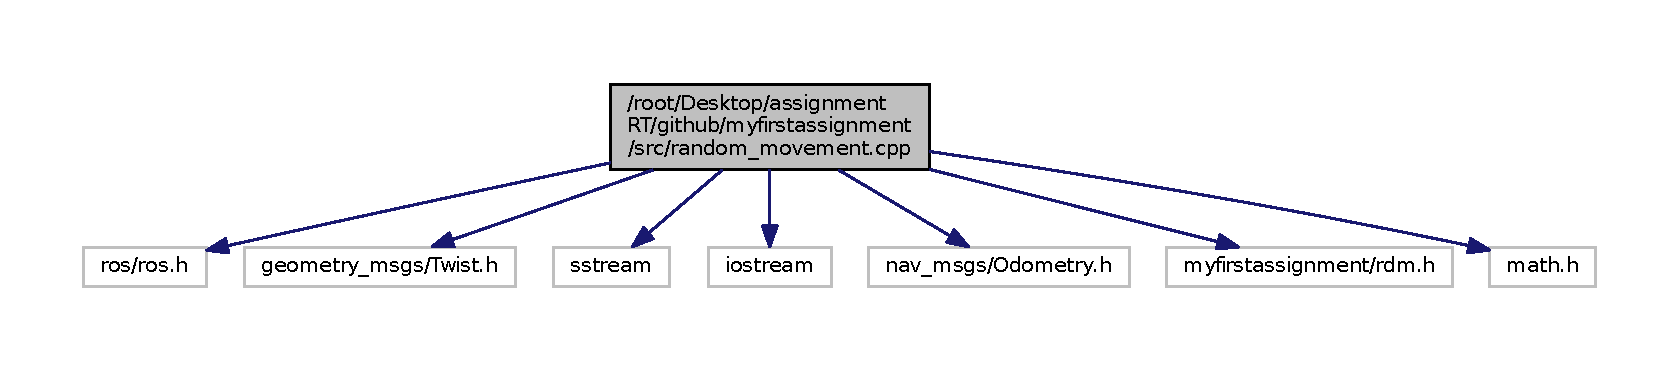
\includegraphics[width=350pt]{random__movement_8cpp__incl}
\end{center}
\end{figure}
\subsection*{Functions}
\begin{DoxyCompactItemize}
\item 
int \hyperlink{random__movement_8cpp_abc69a0e42840344c22a4a74b656eb377}{distance\+\_\+btw\+\_\+points} (int a, int b)
\begin{DoxyCompactList}\small\item\em This function, given two points a and b, provides the euclidean distance between them. \end{DoxyCompactList}\item 
void \hyperlink{random__movement_8cpp_aef70658f8ec02213922917e67d9e1c76}{subscriber\+Callback} (const nav\+\_\+msgs\+::\+Odometry\+::\+Const\+Ptr \&pose\+\_\+msg)
\begin{DoxyCompactList}\small\item\em This function, is called every time something is read from the topic /odom. \end{DoxyCompactList}\item 
int \hyperlink{random__movement_8cpp_a3c04138a5bfe5d72780bb7e82a18e627}{main} (int argc, char $\ast$$\ast$argv)
\end{DoxyCompactItemize}
\subsection*{Variables}
\begin{DoxyCompactItemize}
\item 
ros\+::\+Publisher \hyperlink{random__movement_8cpp_a350594df3e8f6948c8462edfd41ce086}{pub}
\item 
ros\+::\+Service\+Client \hyperlink{random__movement_8cpp_a17bcd065930a8a7f9f194078d9977268}{client}
\item 
myfirstassignment\+::rdm \hyperlink{random__movement_8cpp_a7b452f070094b469cfdb9ed3f7e144ef}{rand\+\_\+position}
\end{DoxyCompactItemize}


\subsection{Function Documentation}
\index{random\+\_\+movement.\+cpp@{random\+\_\+movement.\+cpp}!distance\+\_\+btw\+\_\+points@{distance\+\_\+btw\+\_\+points}}
\index{distance\+\_\+btw\+\_\+points@{distance\+\_\+btw\+\_\+points}!random\+\_\+movement.\+cpp@{random\+\_\+movement.\+cpp}}
\subsubsection[{\texorpdfstring{distance\+\_\+btw\+\_\+points(int a, int b)}{distance_btw_points(int a, int b)}}]{\setlength{\rightskip}{0pt plus 5cm}int distance\+\_\+btw\+\_\+points (
\begin{DoxyParamCaption}
\item[{int}]{a, }
\item[{int}]{b}
\end{DoxyParamCaption}
)}\hypertarget{random__movement_8cpp_abc69a0e42840344c22a4a74b656eb377}{}\label{random__movement_8cpp_abc69a0e42840344c22a4a74b656eb377}


This function, given two points a and b, provides the euclidean distance between them. 


\begin{DoxyParams}{Parameters}
{\em a} & is the minimum number of the interval \\
\hline
{\em b} & is the maximum number of the interval \\
\hline
\end{DoxyParams}

\begin{DoxyRetVals}{Return values}
{\em the} & distance (int) between a and b \\
\hline
\end{DoxyRetVals}


Definition at line 32 of file random\+\_\+movement.\+cpp.

\index{random\+\_\+movement.\+cpp@{random\+\_\+movement.\+cpp}!main@{main}}
\index{main@{main}!random\+\_\+movement.\+cpp@{random\+\_\+movement.\+cpp}}
\subsubsection[{\texorpdfstring{main(int argc, char $\ast$$\ast$argv)}{main(int argc, char **argv)}}]{\setlength{\rightskip}{0pt plus 5cm}int main (
\begin{DoxyParamCaption}
\item[{int}]{argc, }
\item[{char $\ast$$\ast$}]{argv}
\end{DoxyParamCaption}
)}\hypertarget{random__movement_8cpp_a3c04138a5bfe5d72780bb7e82a18e627}{}\label{random__movement_8cpp_a3c04138a5bfe5d72780bb7e82a18e627}


Definition at line 83 of file random\+\_\+movement.\+cpp.

\index{random\+\_\+movement.\+cpp@{random\+\_\+movement.\+cpp}!subscriber\+Callback@{subscriber\+Callback}}
\index{subscriber\+Callback@{subscriber\+Callback}!random\+\_\+movement.\+cpp@{random\+\_\+movement.\+cpp}}
\subsubsection[{\texorpdfstring{subscriber\+Callback(const nav\+\_\+msgs\+::\+Odometry\+::\+Const\+Ptr \&pose\+\_\+msg)}{subscriberCallback(const nav_msgs::Odometry::ConstPtr &pose_msg)}}]{\setlength{\rightskip}{0pt plus 5cm}void subscriber\+Callback (
\begin{DoxyParamCaption}
\item[{const nav\+\_\+msgs\+::\+Odometry\+::\+Const\+Ptr \&}]{pose\+\_\+msg}
\end{DoxyParamCaption}
)}\hypertarget{random__movement_8cpp_aef70658f8ec02213922917e67d9e1c76}{}\label{random__movement_8cpp_aef70658f8ec02213922917e67d9e1c76}


This function, is called every time something is read from the topic /odom. 


\begin{DoxyParams}{Parameters}
{\em pose\+\_\+msf} & \\
\hline
{\em } & \\
\hline
\end{DoxyParams}


Definition at line 43 of file random\+\_\+movement.\+cpp.



\subsection{Variable Documentation}
\index{random\+\_\+movement.\+cpp@{random\+\_\+movement.\+cpp}!client@{client}}
\index{client@{client}!random\+\_\+movement.\+cpp@{random\+\_\+movement.\+cpp}}
\subsubsection[{\texorpdfstring{client}{client}}]{\setlength{\rightskip}{0pt plus 5cm}ros\+::\+Service\+Client client}\hypertarget{random__movement_8cpp_a17bcd065930a8a7f9f194078d9977268}{}\label{random__movement_8cpp_a17bcd065930a8a7f9f194078d9977268}


Definition at line 22 of file random\+\_\+movement.\+cpp.

\index{random\+\_\+movement.\+cpp@{random\+\_\+movement.\+cpp}!pub@{pub}}
\index{pub@{pub}!random\+\_\+movement.\+cpp@{random\+\_\+movement.\+cpp}}
\subsubsection[{\texorpdfstring{pub}{pub}}]{\setlength{\rightskip}{0pt plus 5cm}ros\+::\+Publisher pub}\hypertarget{random__movement_8cpp_a350594df3e8f6948c8462edfd41ce086}{}\label{random__movement_8cpp_a350594df3e8f6948c8462edfd41ce086}


Definition at line 20 of file random\+\_\+movement.\+cpp.

\index{random\+\_\+movement.\+cpp@{random\+\_\+movement.\+cpp}!rand\+\_\+position@{rand\+\_\+position}}
\index{rand\+\_\+position@{rand\+\_\+position}!random\+\_\+movement.\+cpp@{random\+\_\+movement.\+cpp}}
\subsubsection[{\texorpdfstring{rand\+\_\+position}{rand_position}}]{\setlength{\rightskip}{0pt plus 5cm}myfirstassignment\+::rdm rand\+\_\+position}\hypertarget{random__movement_8cpp_a7b452f070094b469cfdb9ed3f7e144ef}{}\label{random__movement_8cpp_a7b452f070094b469cfdb9ed3f7e144ef}


Definition at line 24 of file random\+\_\+movement.\+cpp.


\hypertarget{random__service_8cpp}{}\section{/root/\+Desktop/assignment\+R\+T/github/myfirstassignment/src/random\+\_\+service.cpp File Reference}
\label{random__service_8cpp}\index{/root/\+Desktop/assignment\+R\+T/github/myfirstassignment/src/random\+\_\+service.\+cpp@{/root/\+Desktop/assignment\+R\+T/github/myfirstassignment/src/random\+\_\+service.\+cpp}}
{\ttfamily \#include \char`\"{}ros/ros.\+h\char`\"{}}\\*
{\ttfamily \#include \char`\"{}myfirstassignment/rdm.\+h\char`\"{}}\\*
{\ttfamily \#include $<$math.\+h$>$}\\*
Include dependency graph for random\+\_\+service.\+cpp\+:\nopagebreak
\begin{figure}[H]
\begin{center}
\leavevmode
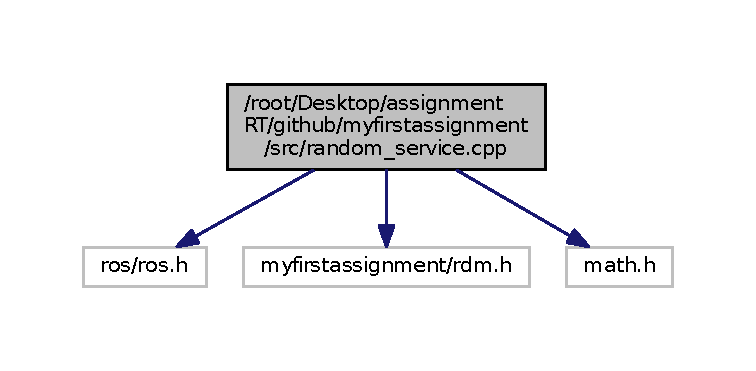
\includegraphics[width=350pt]{random__service_8cpp__incl}
\end{center}
\end{figure}
\subsection*{Functions}
\begin{DoxyCompactItemize}
\item 
bool \hyperlink{random__service_8cpp_ae81a0ba2bef3c9a93c7b8df4d00b7e16}{Rand} (myfirstassignment\+::rdm\+::\+Request \&req, myfirstassignment\+::rdm\+::\+Response \&res)
\begin{DoxyCompactList}\small\item\em This function is called under request. It ask for a request and returns the target\textquotesingle{}s coordinates. \end{DoxyCompactList}\item 
int \hyperlink{random__service_8cpp_a3c04138a5bfe5d72780bb7e82a18e627}{main} (int argc, char $\ast$$\ast$argv)
\end{DoxyCompactItemize}


\subsection{Function Documentation}
\index{random\+\_\+service.\+cpp@{random\+\_\+service.\+cpp}!main@{main}}
\index{main@{main}!random\+\_\+service.\+cpp@{random\+\_\+service.\+cpp}}
\subsubsection[{\texorpdfstring{main(int argc, char $\ast$$\ast$argv)}{main(int argc, char **argv)}}]{\setlength{\rightskip}{0pt plus 5cm}int main (
\begin{DoxyParamCaption}
\item[{int}]{argc, }
\item[{char $\ast$$\ast$}]{argv}
\end{DoxyParamCaption}
)}\hypertarget{random__service_8cpp_a3c04138a5bfe5d72780bb7e82a18e627}{}\label{random__service_8cpp_a3c04138a5bfe5d72780bb7e82a18e627}


Definition at line 33 of file random\+\_\+service.\+cpp.

\index{random\+\_\+service.\+cpp@{random\+\_\+service.\+cpp}!Rand@{Rand}}
\index{Rand@{Rand}!random\+\_\+service.\+cpp@{random\+\_\+service.\+cpp}}
\subsubsection[{\texorpdfstring{Rand(myfirstassignment\+::rdm\+::\+Request \&req, myfirstassignment\+::rdm\+::\+Response \&res)}{Rand(myfirstassignment::rdm::Request &req, myfirstassignment::rdm::Response &res)}}]{\setlength{\rightskip}{0pt plus 5cm}bool Rand (
\begin{DoxyParamCaption}
\item[{myfirstassignment\+::rdm\+::\+Request \&}]{req, }
\item[{myfirstassignment\+::rdm\+::\+Response \&}]{res}
\end{DoxyParamCaption}
)}\hypertarget{random__service_8cpp_ae81a0ba2bef3c9a93c7b8df4d00b7e16}{}\label{random__service_8cpp_ae81a0ba2bef3c9a93c7b8df4d00b7e16}


This function is called under request. It ask for a request and returns the target\textquotesingle{}s coordinates. 


\begin{DoxyParams}{Parameters}
{\em req} & the request received from the client (none) \\
\hline
{\em res} & the response returned to the clien (the random coordinates within a specific interval) \\
\hline
\end{DoxyParams}

\begin{DoxyRetVals}{Return values}
{\em the} & random number (True or False) \\
\hline
\end{DoxyRetVals}


Definition at line 23 of file random\+\_\+service.\+cpp.


%--- End generated contents ---

% Index
\backmatter
\newpage
\phantomsection
\clearemptydoublepage
\addcontentsline{toc}{chapter}{Index}
\printindex

\end{document}
